%-------------------------------------------------------------------------------
%-------------------------------------------------------------------------------
%-------------------------------------------------------------------------------
\chapter{Algorithme de Knuth-Morris-Pratt}
%-------------------------------------------------------------------------------
%-------------------------------------------------------------------------------
\thispagestyle{empty}
%-------------------------------------------------------------------------------
%-------------------------------------------------------------------------------
\vskip -1cm

{\sf Dans le T.P. précédent nous avons recherché des motifs, les codons {\sc start} et {\sc stop} dans une chaînd d'ADN. Cette recherche est un outil important. Par exemple, en génétique, on utilise des algorithmes de recherche pour identifier les similarités entre deux séquences d’ADN. Pour cela, on procède de la manière suivante :
\begin{itemize}
    \item découper la première séquence d’ADN en morceaux de taille 50,
    \item rechercher chaque morceau dans la deuxième séquence d’ADN.
\end{itemize}
Une séquence d’ADN est composée de $3.10^9$ caractères.
}

Dans ce TP, \type{chaine} représente une chaîne de caractères dont la longueur sera calculée par \type{n = len(chaine)} et \type{motif} représente une chaîne de caractères dont la longueur sera calculée par \type{p = len(motif)}. On supposera qu'on a toujours $p < n$.

On cherche les occurrences de \type{motif} dans \type{chaine} qui seront symbolisées par les entiers $i$ tels que 
\begin{lstlisting}
motif == chaine{i : i+p]
\end{lstlisting}

Les occurrences de \type{"ACTG"} dans dans \type{"AACTGTCAGGACTATCGTACTG"} se situent aux indices 1et 18.
%-------------------------------------------------------------------------------
%-------------------------------------------------------------------------------
\subsubsection{Algorithme naïf}
%-------------------------------------------------------------------------------
%-------------------------------------------------------------------------------
\begin{Exercise}\it 
Quelle est la valeur maximale d'un indice $i$ en lequel le motif peut apparaître dans la chaîne ? 

En déduire une fonction \type{occurrences1(chaine, motif)} qui renvoie la liste des indices des occurrences du motif dans la chaîne.
\end{Exercise}
%-------------------------------------------------------------------------------
\begin{Answer}
Le dernier caractère du motif sera comparé au terme de la chaîne à la position $i + p - 1$ donc on doit avoit $i+p-1 \le n-1$ : $i \le n-p$. Bien sur on doit avoir $i\ge 0$.
\begin{lstlisting}
def occurrences(chaine, motif):
    n = len(chaine)
    p = len(motif)
    occ = []
    for i in range(n-p+1):
        if chaine[i : i+p] == motif:
            occ.append(i)
    return occ
\end{lstlisting}
\end{Answer}
%-------------------------------------------------------------------------------
%-------------------------------------------------------------------------------

Dans cet algorithme, on recopie les caractères de la chaîne lors de l'extraction : on effectue donc $p.(n-p+1)$ copies d'un caractère. On va essayer de réduire ce nombre d'opérations.
%-------------------------------------------------------------------------------
\newpage
%-------------------------------------------------------------------------------
\subsubsection{Une amélioration}
%-------------------------------------------------------------------------------
%-------------------------------------------------------------------------------
Plutôt que de copier les caractères et demander à Python de comparer les chaînes on peut comparer les caractères un par un. On pourra cesser la comparaison dès qu'on a trouvé une différence.
%--------------------------------------------------------------------------
\begin{lstlisting}
pour chaque i possible
    pour chaque k entre 0 et p-1
        on compare chaine[i+k] et motif[k]
            on renvoie False si les caractères sont distincts
on renvoie True
\end{lstlisting}
%--------------------------------------------------------------------------
\begin{center}
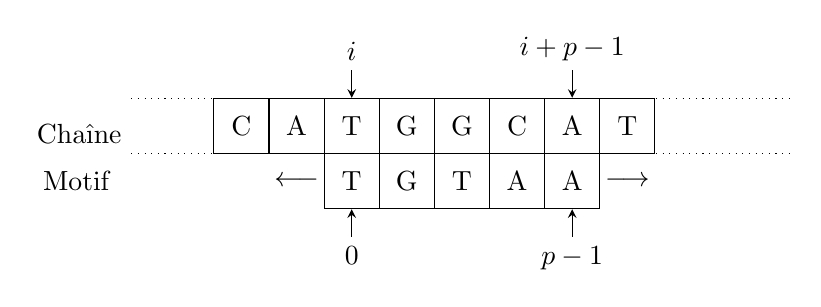
\begin{tikzpicture}[>=stealth, scale=0.7]
\tikzstyle{case}=[rectangle,draw,minimum size =7mm,fill=white]
\draw[dotted] (-4,-0.5) node[above left]{Chaîne} -- +(12, 0);
\draw[dotted] (-4,0.5)  -- +(12,0);
\node[case](cb) at (-2,0) {C};
\node[case](ca) at (-1,0) {A};
\node[case](c0) at (0,0) {T};
\node[case](c1) at (1,0) {G};
\node[case](c2) at (2,0) {G};
\node[case](c3) at (3,0) {C};
\node[case](c4) at (4,0) {A};
\node[case](c5) at (5,0) {T};
\node   at (-5, -1) {Motif};
\node   at (-1, -1) {$\longleftarrow$};
\node[case](m0) at (0,-1) {T};
\node[case](m1) at (1,-1) {G};
\node[case](m2) at (2,-1) {T};
\node[case](m3) at (3,-1) {A};
\node[case](m4) at (4,-1) {A};
\node   at (5, -1) {$\longrightarrow$};
\draw[<-] (c0.north) -- +(0, 0.5) node[above]{$i$};
\draw[<-] (c4.north) -- +(0, 0.5) node[above]{$i+p-1$};
\draw[<-] (m0.south) -- +(0, -0.5) node[below]{$0$};
\draw[<-] (m4.south) -- +(0, -0.5) node[below]{$p-1$};
\end{tikzpicture}
\end{center}
%--------------------------------------------------------------------------
Dans cet exemple on voit une différence à la troisième comparaison, on n'a pas une occurence du motif.

%-------------------------------------------------------------------------------
%-------------------------------------------------------------------------------
\begin{Exercise}\it 
En déduire une fonction \type{occurrences2(chaine, motif)} qui renvoie la liste des indices des occurrences du motif dans la chaîne en utilisant cette méthode.
\end{Exercise}
%-------------------------------------------------------------------------------
\begin{Answer}
Le dernier caractère du motif sera comparé au terme de la chaîne à la position $i + p - 1$ donc on doit avoit $i+p-1 \le n-1$ : $i \le n-p$. Bien sur on doit avoir $i\ge 0$.
\begin{lstlisting}
def occurrences(chaine, motif):
    n = len(chaine)
    p = len(motif)
    occ = []
    for i in range(n-p+1):
        if chaine[i : i+p] == motif:
            occ.append(i)
    return occ
\end{lstlisting}
\end{Answer}
%-------------------------------------------------------------------------------
%-------------------------------------------------------------------------------
%-------------------------------------------------------------------------------
%-------------------------------------------------------------------------------
\begin{Exercise}[title = Statistiques]\it 
Écrire une fonction \type{composition(chaine)} qui renvoie les statistiques de \type{chaine} : nombre d’occurrences et pourcentage de chaque caractère.
\end{Exercise}
%-------------------------------------------------------------------------------
\begin{Answer}
On peut fixer le format des nombres utilisés dans la méthode \type{format} :

\type{:3d} écrit un entier avec 3 emplacements

\type{:5.2f} écrit un flottant avec 5 emplacements (y compris le point de séparation) avec 2 chiffres après la vigule.

\begin{lstlisting}
def composition(chaine):
   n = len(chaine)
   print('La chaîne', chaine, 'contient')
   for lettre in 'ACGT':
       k = nb_lettres(chaine, lettre)
       print('{:2d} fois {}, soit {:5.2f} %'.format(k, lettre, k/n*100))
\end{lstlisting}
\end{Answer}
%-------------------------------------------------------------------------------
%-------------------------------------------------------------------------------
\begin{lstlisting}
La chaîne GATGCATTAGTAAGGGGTAGA contient
 7 fois A, soit 33.33 %
 1 fois C, soit  4.76 %
 8 fois G, soit 38.10 %
 5 fois T, soit 23.81 %
\end{lstlisting}
%-------------------------------------------------------------------------------
%-------------------------------------------------------------------------------
\begin{Exercise}\it 
Écrire une fonction \type{renverse(chaine)} qui prend comme argument une chaîne de caractères et la renvoie dans l'ordre inverse.
\end{Exercise}
%-------------------------------------------------------------------------------
\begin{Answer}
On prend les caractères dans l'ordre et on les ajoute à gauche depuis une chaîne vide.

\begin{lstlisting}
def renverse(chaine):
    eniahc = ""
    for car in chaine:
       eniahc = car + eniahc
    return eniahc
\end{lstlisting}
\end{Answer}
%-------------------------------------------------------------------------------
%-------------------------------------------------------------------------------
\type{renverse(ch0)} renverra \type{'AGATGGGGAATGATTACGTAG'}.
%-------------------------------------------------------------------------------
%-------------------------------------------------------------------------------
\subsubsection{Mutations}
%-------------------------------------------------------------------------------
%-------------------------------------------------------------------------------
{\sf Une mutation est une modification de l'information génétique dans le génome d'une cellule ou d'un virus et par conséquent une modification de la séquence de l'ADN. 

Les mutations sont une des causes principales de l'évolution des espèces.} 
%-------------------------------------------------------------------------------
%-------------------------------------------------------------------------------
\begin{Exercise}\it 
Écrire une fonction \type{changement(chaine, k, car)} qui calcule et renvoie une nouvelle chaîne semblable à la chaîne initiale à l'exception du  caractère à la position \type{k} (\type{0 <= k < len(chaine)}) qui est remplacé par \type{car}.
\end{Exercise}
%-------------------------------------------------------------------------------
\begin{Answer}
\begin{lstlisting}
def changement(chaine, k, car):
    return chaine[ :k] + car + chaine[k+1 : ]
\end{lstlisting}
\end{Answer}
%-------------------------------------------------------------------------------
%-------------------------------------------------------------------------------
\type{changement(ch0, 5, 'C')} renverra \type{'GATGCCTTAGTAAGGGGTAGA'}.
%-------------------------------------------------------------------------------
%-------------------------------------------------------------------------------
\begin{Exercise}\it 
Écrire une fonction \type{mutation(chaine)} qui renvoie la chaîne initiale après avoir remplacé un caractère à une position choisie aléatoirement par {\bf un autre} caractère choisi, lui aussi, aléatoirement.
\end{Exercise}
%-------------------------------------------------------------------------------
\begin{Answer}
\begin{lstlisting}
def mutation(chaine):
    n = len(chaine)
    k = rd.randint(0, n-1)
    car = rd.choice('ACGT')
    while car == chaine[k]:
        car = rd.choice('ACGT')
    return changement(chaine, k, car)
\end{lstlisting}
\end{Answer}
%-------------------------------------------------------------------------------
%-------------------------------------------------------------------------------
\type{mutation(ch0)} peut renvoyer \type{'GATGCATTAGTATGGGGTAGA'}.
%-------------------------------------------------------------------------------
%-------------------------------------------------------------------------------

\medskip

La probabilité de mutation d'un nucléotide dans une période d'un million d'année est estimée à $\alpha = 1,5.10^{-2}$.
On approchera le nombre de mutations d'une chaîne de longueur $N$ dans une période de $T$ millions d'années par la partie entière de $\alpha.N.T$. 

Ces mutations peuvent intervenir plus d'une fois sur le même nucléotide : le nombre de nucléotides modifiés peut donc être inférieur au nombre de mutations.
%-------------------------------------------------------------------------------
%-------------------------------------------------------------------------------
\begin{Exercise}\it 
Écrire une fonction \type{mutations(chaine, T)} qui renvoie une chaîne ayant subi les mutations de puis la chaîne initiale, correspondant à une période de $T$ millions d'années.
\end{Exercise}
%-------------------------------------------------------------------------------
\begin{Answer}
\begin{lstlisting}
def mutations(chaine, T):
    alpha = 1.5e-2
    N = len(chaine)
    p = int(alpha*N*T)
    for i in range(p):
        chaine = mutation(chaine)
    return chaine
\end{lstlisting}
\end{Answer}
%-------------------------------------------------------------------------------
%-------------------------------------------------------------------------------
\type{mutations(ch0, 10)} peut renvoyer \type{ch1 = 'GAGGCATCAGTAAGGGGTGGA'}.
\medskip

Il existe des modèles plus sophistiqués de mutation.

Les nucléotides sont décomposées en deux classes : 

les purines (A et G) et les pyrimidines (C et T). 

Les mutations se font plus souvent dans une classe (entre A et G ou entre C et T). Le modèle de Kimura (1980) estime que la probabilité de mutation vers l'élément de la  même classe est $\frac 23$ tandis que la probabilité de mutation vers un des 2 éléments de l'autre classe est de $\frac 16$.
%--------------------------------------------------------------------------
\begin{Exercise}[title = Question facultative]\it 
Écrire une fonction \type{mutationsK(chaine)} qui renvoie la chaîne initiale après avoir remplacé un caractère à une position choisie aléatoirement par caractère choisi selon le modèle de Kimura.
\end{Exercise}
%-------------------------------------------------------------------------------
\begin{Answer}
On commence par déterminer les choix possibles à partir d'un nucléotide : l'élément de la même classe apparaît 4 fois pour avoir une probabilité de tirage de $\frac 46=\frac 23$
\begin{lstlisting}
def choix(car):
    if car  == "A":
        return 'GGGGCT'
    elif car  == "C":
        return 'TTTTAG'
    elif car  == "G":
        return 'AAAACT'
    else:
        return 'CCCCAG'
\end{lstlisting}

\begin{lstlisting}
def mutationK(chaine):
    n = len(chaine)
    k = rd.randint(0, n-1)
    car = rd.choice(choix(chaine[k]))
    return changement(chaine, k, car)
\end{lstlisting}

\begin{lstlisting}
def mutationsK(chaine, T):
    alpha = 1.5e-2
    N = len(chaine)
    p = int(alpha*N*T)
    for i in range(p):
        chaine = mutation(chaine)
    return chaine
\end{lstlisting}

\end{Answer}
%-------------------------------------------------------------------------------
%-------------------------------------------------------------------------------
\begin{Exercise}\it 
Écrire une fonction \type{difference(ch1, ch2)} où \type{ch1} et \type{ch2} ont même longueur qui calcule une troisième chaîne, de même longueur, contenant un espace aux positions où il n'y a pas eu mutation, et un \type{X} là où il y a une différence entre \type{ch1} et \type{ch2}. La fonction imprimera ensuite les trois chaînes en les alignant pour bien repérer les mutations et contrôler les fonctions.
\end{Exercise}
%-------------------------------------------------------------------------------
\begin{Answer}
\begin{lstlisting}
def difference(ch1, ch2):
    n = len(ch1)
    diff = ""
    for i in range(n):
        if ch1[i] != ch2[i]:
            diff = diff + 'X'
        else:
            diff = diff + ' '
    print(ch1)
    print(ch2)
    print(diff)
\end{lstlisting}
\end{Answer}
%-------------------------------------------------------------------------------
%-------------------------------------------------------------------------------
\type{difference(ch0, ch1)} imprimera
\begin{lstlisting}
GATGCATTAGTAAGGGGTAGA
GAGGCATCAGTAAGGGGTGGA
  X    X          X  
  \end{lstlisting}
%-------------------------------------------------------------------------------
%-------------------------------------------------------------------------------
\subsubsection{Recherche des séquences codantes}
%-------------------------------------------------------------------------------
%-------------------------------------------------------------------------------
Dans notre modèle, nous particulariserons quatre séquences de 3 nucléotides (ou {\bf codons}) : le codon ATG appelé {\sc start}, et les codons TAA, TAG et TGA, appelés codons {\sc stop}. Nous définirons une {\bf séquence codante} comme une portion continue de la chaîne telle que :
\begin{itemize}
\item elle commence par un {\sc start} et se termine par un {\sc stop},
\item ce {\sc start} et ce {\sc stop} sont {\bf en phase}, c'est-à-dire qu'ils sont séparés par un nombre de nucléotides multiple de~3.
\end{itemize}
Par exemple, dans la séquence \type{ch0}, il y un codon {\sc start} commençant en 1, et 3 codons {\sc stop}: \type{'TAG'} en 7 et en 17 et \type{'TAA'} en 10. Deux couples sont en phase et correspondent donc à des régions codantes de l'ADN.
%-------------------------------------------------------------------------------
%-------------------------------------------------------------------------------
\begin{Exercise}\it 
Écrire une fonction \type{reperage\_codons} qui parcourt une chaîne ADN, localise et identifie les codons {\sc start} et {\sc stop} en renvoyant deux listes: une liste des indices des positions de la première lettre des codons {\sc start} et un seconde liste des indices des positions de la première lettre de codons {\sc stop}.
\end{Exercise}
%-------------------------------------------------------------------------------
\begin{Answer}
\begin{lstlisting}
def reperage_codons(chaine):
    position_start = []
    position_stop = []
    for i in range(len(chaine)-2):
        codon = chaine[i:i+3]
        if codon =='ATG':
            position_start+=[i]
        if codon == 'TAA' or codon == 'TAG' or codon == 'TGA':
            position_stop += [i]     
    return(position_start, position_stop)
\end{lstlisting}
\end{Answer}
%-------------------------------------------------------------------------------
%-------------------------------------------------------------------------------
\type{reperage\_codons(ch0)} renvoie \type{([1], [7, 10, 17])}.
%-------------------------------------------------------------------------------
%-------------------------------------------------------------------------------
\begin{Exercise}\it 
Écrire une fonction \type{seq\_codantes} qui analyse la sortie de la fonction précédente pour localiser les séquences codantes en les renvoyant sous la forme de la liste des chaînes de caractères comprises (strictement) entre un codon {\sc start} et un codon {\sc stop} en phase. On devra chercher les séquences codantes dans les deux sens de la chaîne.
\end{Exercise}
%-------------------------------------------------------------------------------
\begin{Answer}
\begin{lstlisting}
def seq_codantes(chaine):
    eniahc = renverse(chaine)
    sequences = []
    for ch in [chaine, eniahc]:
        start, stop = reperage_codons(ch)   
        for i in start:
            for j in stop:
                if j > i  and (j-i)%3 == 0:
                    sequences.append(ch[i+3:j])
    return sequences
\end{lstlisting}
\end{Answer}
%-------------------------------------------------------------------------------
%-------------------------------------------------------------------------------
\type{seq\_codantes(ch0)} renvoie  \type{['CAT', 'CATTAG', 'ATTACG']}

\newpage
%--------------------------------------------------------------------------

 